\documentclass[11pt,a4paper]{article}
\usepackage[latin1]{inputenc}
\usepackage[spanish]{babel}
\usepackage{amsmath}
\usepackage{amsfonts}
\usepackage{amssymb}
\usepackage{graphicx}
\usepackage[left=2cm,right=2cm,top=2cm,bottom=2cm]{geometry}
\author{Samuel Caleb Mart�nez Hern�ndez}
\title{Analisis de elementos finitos }
\begin{document}

\includegraphics[scale=1]{EV/logo.png}  \\

\begin{center}
{\Huge Analisis de elementos finitos}
\end{center}\\

\begin{center}
{\Large Samuel Caleb Mart�nez Hern�ndez }
\end{center}\\

\begin{center}
{\Large Ing. Mecatr�nica 6-A}
\end{center}\\

\begin{center}
{\Large Cinem�tica de Robots}
\end{center}\\

\begin{center}
 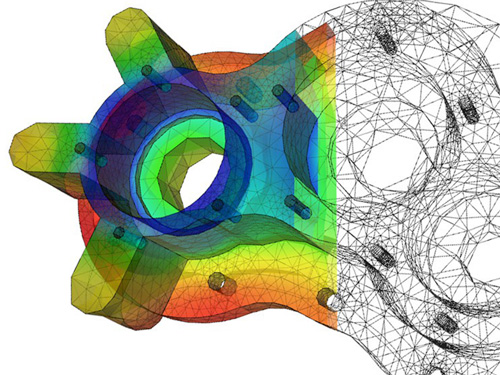
\includegraphics[scale=1]{EV/2.jpg}\\ \\ \\ 
 \end{center} 




\section*{Introducci�n}

Para esta practica vamos a enfocarnos en el an�lisis de elementos finitos y para ello primero debemos explicar de lo que se trata un elemento finito.\\


Pues bien, cuando un elemento es finito en un objeto, en este caso nuestro robot SCARA, se sabe que al ser finito este va a fallar en alg�n momento, en un tiempo y por razones determinadas. Decir todo esto es mas que nada una "predicci�n" por as� decirlo, por ejemplo, cuando tenemos una caja de cart�n y colocamos un objeto considerablemente pesado, sabemos casi por inercia que la dicha caja va a deformarse o 'fallar' como normalmente se le conoce al quebrantamiento de un objeto. \\ 


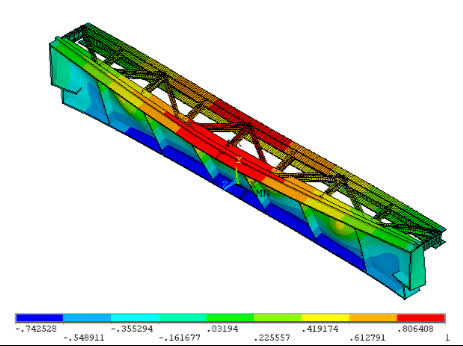
\includegraphics[scale=1]{EV/1.jpg} \\ 


A pesar de haber dicho que esto va a pasar, lo que se espera es todo lo contrario, ya que en el an�lisis de elementos finitos, se hacen comparaciones entre materiales y/o uniones entre piezas, con el fin de saber que material es mejor para cierto trabajo y cuales no. \\


En la imagen anterior podemos observar un objeto con diferentes tonalidades, desde roja a azul, digamos lo as� como ir de un extremo a otro, donde el extremo azul representa la parte del objeto que no presenta cambios ni en su forma ni en integridad, mientras que el extremo rojo nos indica la parte del objeto que ya a sufrido un cambio en su forma y su integridad debido a la fuerza que se le ejerce, las partes medias o sea, las amarillas representan el cambio de estado entre azul y rojo, es decir, tu objeto se esta empezando a romper. \\

Una vez explicado esto, ya podemos pasar al an�lisis de nuestros elementos finitos, dado que ya se tiene el conocimiento necesario para entender de manera considerable lo que ocurre con nuestro robot SCARA y la raz�n de ello. \\ \\


\section*{An�lisis de Elementos Finitos}

Como proyecto, nuestro robot es tipo SCARA, por lo que los brazos que este posee, serna las partes que mayor peso tendr�n que soportar relativamente, ya que en si, la base soportar�a la suma de todas las cargas, pero por ser una base, esta est� dise�ada para soportar todo el robot entero, por lo que corre menos riesgo de romperse, las partes del brazo, son las que llevan la carga mas 'peligrosa' dado que estas 'penden' y no es que tengan algo que las sujete directamente mas que su propia uni�n entre pieza y pieza.\\ 

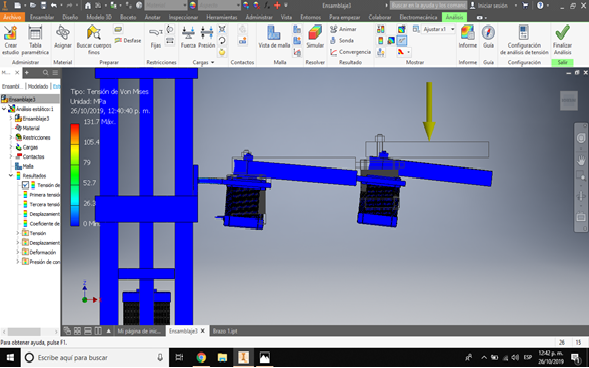
\includegraphics[scale=1]{EV/3.png} \\

Al realizar en an�lisis de elementos, pudimos ver que contamos con una base bastante resistente en casi todos los sentidos, aun as�, nos percatamos de que la parte del brazo es la mas propensa a fallar, dado que la gravedad juega en su contra, sin contar claro con el peso adicional que se le sume.\\

Sabemos que este pandeo no se debe tanto por le material de las piezas, si no por la propia forma del brazo en general, a cualquiera le resultar�a bastante l�gico que al someter algo que pende a una fuerza, la punta empezar� a pandearse con el tiempo, hasta ese punto, es comprensible que ocurra eso. \\

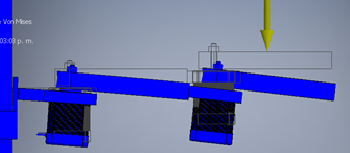
\includegraphics[scale=1]{EV/4.png} \\

Se ha intentado hacer an�lisis con toda la lista disponible de materiales con la que cuenta INVENTOR, sin embargo, en todas y cada una parece darnos el mismo resultado, por lo cual, dimos a la conclusi�n de que tendr�amos que hacer un nuevo an�lisis y dar con el origen de la falla. \\

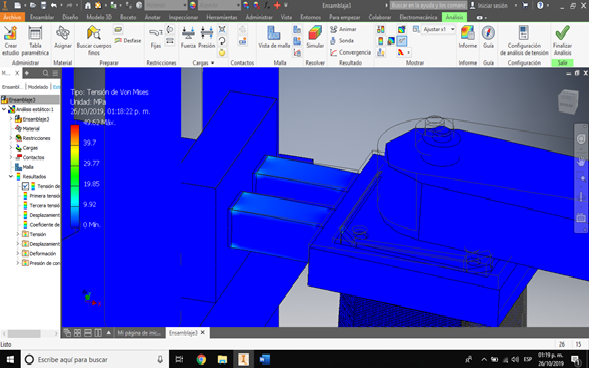
\includegraphics[scale=1]{EV/5.png} \\

Analizando de la manera mas meticulosa, por fin, encontramos el origen de la falla, y no es que se trate del materia, ni siquiera de la fuerza que se le ejerce (que no es mucha), si no que se trata de la uni�n entre la base y el brazo del robot, la cual resulta ser bastante d�bil. \\

La debilidad de la uni�n entre el brazo y la base, es la principal causante de la falla en el robot. Como soluci�n, sera dise�ar una uni�n mucho mas fuerte y resistente, dado que termina siendo de las partes del robot que mas fuerza requieren tener. \\

Casi al finalizar, se realizara un ultimo an�lisis de elementos, agregando la fuerza que le ejercer�n los motores con su peso. \\

\section*{Conclusi�n}

La forma original del robot resulta ser perjudicial para este, si no se tiene una uni�n lo suficientemente fuerte como para soportar la parte que va a pender, ya que como ya se ha comentado, es la parte que menos estar� en equilibro, por lo tanto, estar� muy a costa de la gravedad y el peso de los objetos que tenga que cargar. \\


\section*{Referencias}\\

@book{lizarza2000metodo,
  title={M{\'e}todo de los elementos finitos para an{\'a}lisis estructural},
  author={Lizarza, Juan Tom{\'a}s Celig{\"u}eta},
  year={2000},
  publisher={Escuela Superior de Ingeniros Industriales, Universidad de Navarra}
}








\end{document}